% GovAllocXAI v2 -- CONFERENCE paper (IEEEtran, two columns). Compiles on Overleaf: pdflatex, bibtex, pdflatex x2. Target length: 6 pages.
\documentclass[conference]{IEEEtran}
\usepackage[T1]{fontenc}
\usepackage[utf8]{inputenc}
\usepackage{amsmath,amssymb}
\usepackage{graphicx,booktabs,xcolor}
\usepackage{url}
\usepackage{cite}
\makeatletter\renewcommand{\fps@table}{!t}\expandafter\def\csname fps@table*\endcsname{!t}\makeatother
% Macros regenerated by pipeline/27_make_figures_tables.py - do not edit by hand
\newcommand{\NMasterRows}{5{,}450}
\newcommand{\NMasterCols}{217}
\newcommand{\NMasterCountries}{217}
\newcommand{\NCofogRows}{825}
\newcommand{\NCofogCountries}{36}
\newcommand{\NWdiRows}{4{,}995}
\newcommand{\NWdiCountries}{211}
\newcommand{\NLegacyMatched}{750}
\newcommand{\NOecdAdded}{6}
\newcommand{\NOecdRowsComplete}{109}
\newcommand{\NOverlapRows}{690}
\newcommand{\NXsrcMedDiff}{0.025}
\newcommand{\NXsrcMinR}{0.996}
\newcommand{\NWdiIndicators}{26}
\newcommand{\NFeatNum}{30}
\newcommand{\NFeatModel}{25}
\newcommand{\NSlsqpDiff}{3.6e-15}
\newcommand{\ResTVDPersist}{3.62}
\newcommand{\ResTVDPersistLo}{3.17}
\newcommand{\ResTVDPersistHi}{4.08}
\newcommand{\ResTVDHyb}{3.48}
\newcommand{\ResTVDHybLo}{3.06}
\newcommand{\ResTVDHybHi}{3.91}
\newcommand{\ResTVDCountryMean}{6.96}
\newcommand{\ResPairedGain}{0.140}
\newcommand{\ResPairedLo}{0.025}
\newcommand{\ResPairedHi}{0.277}
\newcommand{\ResRowsImproved}{53}
\newcommand{\ResColdHyb}{10.77}
\newcommand{\ResColdHybLo}{9.60}
\newcommand{\ResColdHybHi}{12.05}
\newcommand{\ResColdPeer}{11.34}
\newcommand{\ResColdGlobal}{11.35}
\newcommand{\ResColdGain}{0.35}
\newcommand{\ResColdGainLo}{-0.44}
\newcommand{\ResColdGainHi}{1.10}
\newcommand{\ATest}{178}
\newcommand{\ATrain}{611}
\newcommand{\AYearLo}{2000}
\newcommand{\AYearHi}{2024}
\newcommand{\LegXGBR}{0.996}
\newcommand{\LegFormulaR}{0.924}
\newcommand{\LegConstRatioR}{-0.011}
\newcommand{\LegNConst}{11}
\newcommand{\LegNIdent}{12}
\newcommand{\LegHealthWith}{0.987}
\newcommand{\LegHealthWithout}{0.969}
\newcommand{\LegTempXGB}{0.945}
\newcommand{\LegTempFormula}{0.932}
\newcommand{\EngTVDBefore}{3.48}
\newcommand{\AgrHealthRho}{0.58}
\newcommand{\AgrSocialProtectionRho}{0.64}
\newcommand{\AgrDefenceRho}{0.52}
\newcommand{\AgrEducationRho}{0.67}
\newcommand{\AgrTransportRho}{0.59}
\newcommand{\AgrGeneralPublicServicesRho}{0.56}
\newcommand{\AgrRhoMean}{0.59}
\newcommand{\AgrJacMean}{0.48}
\newcommand{\AgrSignMean}{0.85}
\newcommand{\AgrLimeFit}{0.52}
\newcommand{\AgrStabMean}{0.86}
\newcommand{\AgrFaithMean}{3.1}
\newcommand{\AgrFaithMin}{2.0}
\newcommand{\AgrFaithMax}{3.8}
\newcommand{\LegXGBRConst}{0.9991}
\newcommand{\LegFormulaRConst}{0.9997}
\newcommand{\LegRealXGB}{0.987}
\newcommand{\LegRealFormula}{0.714}
\newcommand{\LegConstRatioConst}{-0.0002}
\newcommand{\LegXGBRatioConst}{0.88}
\newcommand{\FSStackTenGain}{1.26}
\newcommand{\FSStackTenLo}{0.68}
\newcommand{\FSStackTenHi}{1.84}
\newcommand{\FSStackTenHolm}{0.0008}
\newcommand{\FSStackSixteenGain}{0.81}
\newcommand{\FSStackSixteenLo}{0.20}
\newcommand{\FSStackSixteenHi}{1.34}
\newcommand{\FSStackSixteenHolm}{0.060}
\newcommand{\FSXgbTenGain}{0.89}
\newcommand{\FSXgbTenLo}{0.19}
\newcommand{\FSXgbTenHi}{1.58}
\newcommand{\FSXgbTenHolm}{0.060}
\newcommand{\FSXgbSixteenGain}{0.47}
\newcommand{\FSXgbSixteenLo}{-0.22}
\newcommand{\FSXgbSixteenHi}{1.13}
\newcommand{\FSXgbSixteenHolm}{0.171}
\newcommand{\FSKnnTenGain}{1.25}
\newcommand{\FSKnnTenLo}{0.71}
\newcommand{\FSKnnTenHi}{1.78}
\newcommand{\FSKnnTenHolm}{0.0008}
\newcommand{\FSKnnSixteenGain}{0.66}
\newcommand{\FSKnnSixteenLo}{0.19}
\newcommand{\FSKnnSixteenHi}{1.14}
\newcommand{\FSKnnSixteenHolm}{0.034}
\newcommand{\FSStackXgbTenGain}{0.38}
\newcommand{\FSStackXgbTenLo}{0.06}
\newcommand{\FSStackXgbTenHi}{0.69}
\newcommand{\FSStackXgbTenHolm}{0.060}
\newcommand{\FSStackXgbSixteenGain}{0.34}
\newcommand{\FSStackXgbSixteenLo}{-0.03}
\newcommand{\FSStackXgbSixteenHi}{0.71}
\newcommand{\FSStackXgbSixteenHolm}{0.140}
\newcommand{\FSTVDPeerTen}{14.99}
\newcommand{\FSTVDStackTen}{13.73}
\newcommand{\FSTVDKnnTen}{13.74}
\newcommand{\FSTVDPeerSixteen}{11.31}
\newcommand{\FSTVDStackSixteen}{10.50}
\newcommand{\ResidualMean}{2.6}
\newcommand{\ResidualMedian}{1.8}
\newcommand{\ResidualMax}{29.7}
\newcommand{\AnnSeedMeanGain}{0.12}
\newcommand{\AnnSeedMinGain}{0.10}
\newcommand{\AnnSeedMaxGain}{0.14}
\newcommand{\AnnSeedNExcl}{1}
\newcommand{\AnnSeedN}{5}
\newcommand{\AnnXgbSeedMeanGain}{0.04}
\newcommand{\CovPooledHealth}{0.41}
\newcommand{\CovPooledSocial}{0.31}
\newcommand{\CovPooledEducation}{0.51}
\newcommand{\CovTwentyHealth}{0.27}
\newcommand{\CovTwentySocial}{0.34}
\newcommand{\NTenRows}{1526}
\newcommand{\NTenEcon}{85}
\newcommand{\NTenImf}{623}
\newcommand{\ColdStackSixteen}{10.53}
\newcommand{\ColdPeerSixteen}{11.34}
\newcommand{\ColdStackTen}{13.77}
\newcommand{\ColdStackTenLo}{12.30}
\newcommand{\ColdStackTenHi}{15.45}
\newcommand{\ColdPeerTen}{15.01}
\newcommand{\ColdBestTen}{14.12}
\newcommand{\HistPersistTen}{4.62}
\newcommand{\HistStackTen}{4.82}
\newcommand{\HistBestTen}{4.56}
\newcommand{\NovRho}{0.70}
\newcommand{\ErrHigh}{11.4}
\newcommand{\ErrLow}{33.4}
\newcommand{\ErrLowerMid}{22.0}
\newcommand{\HistStackSixteen}{3.50}
\newcommand{\TotPersist}{2.87}
\newcommand{\TotDeltaRidge}{1.83}
\newcommand{\TotColdMean}{5.63}
\newcommand{\TotColdRidge}{3.82}

% Figures for the conference version (two-column IEEE). Each is a macro called once, next to the text that first discusses it.
\newcommand{\figArch}{\begin{figure*}[!t]
\centering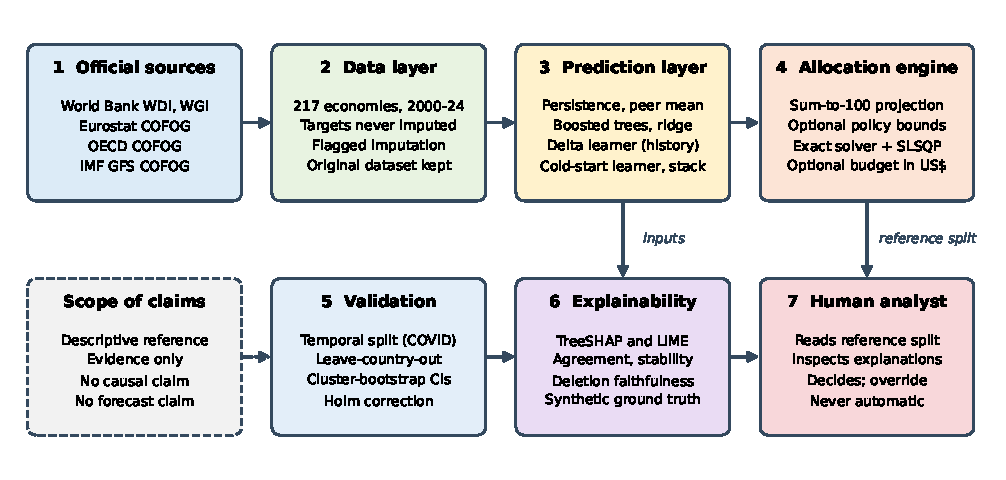
\includegraphics[width=0.85\textwidth]{figures/fig1_architecture.pdf}
\caption{Evaluated components of GovAllocXAI: official sources, flagged data layer, history-based and cold-start learners, bounded-simplex projection, explanation and validation layers; the intended user is a human analyst.}\label{fig:arch}
\end{figure*}}
\newcommand{\figAudit}{\begin{figure*}[!t]
\centering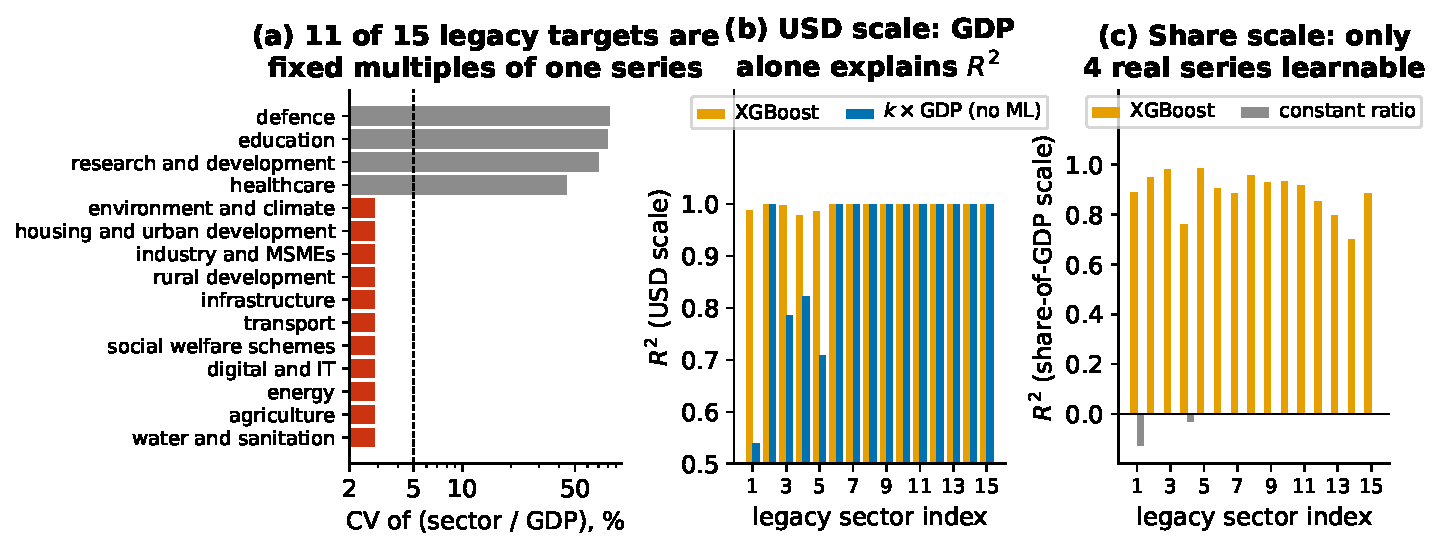
\includegraphics[width=\textwidth]{figures/fig3_legacy_audit.pdf}
\caption{Forensic audit of the legacy v1 benchmark: (a) eleven sectors are fixed multiples of one series; (b) $k\times$GDP matches XGBoost on them (USD scale); (c) a constant-share predictor has $R^2\approx0$ (share scale).}\label{fig:audit}
\end{figure*}}
\newcommand{\figMain}{\begin{figure*}[!t]
\centering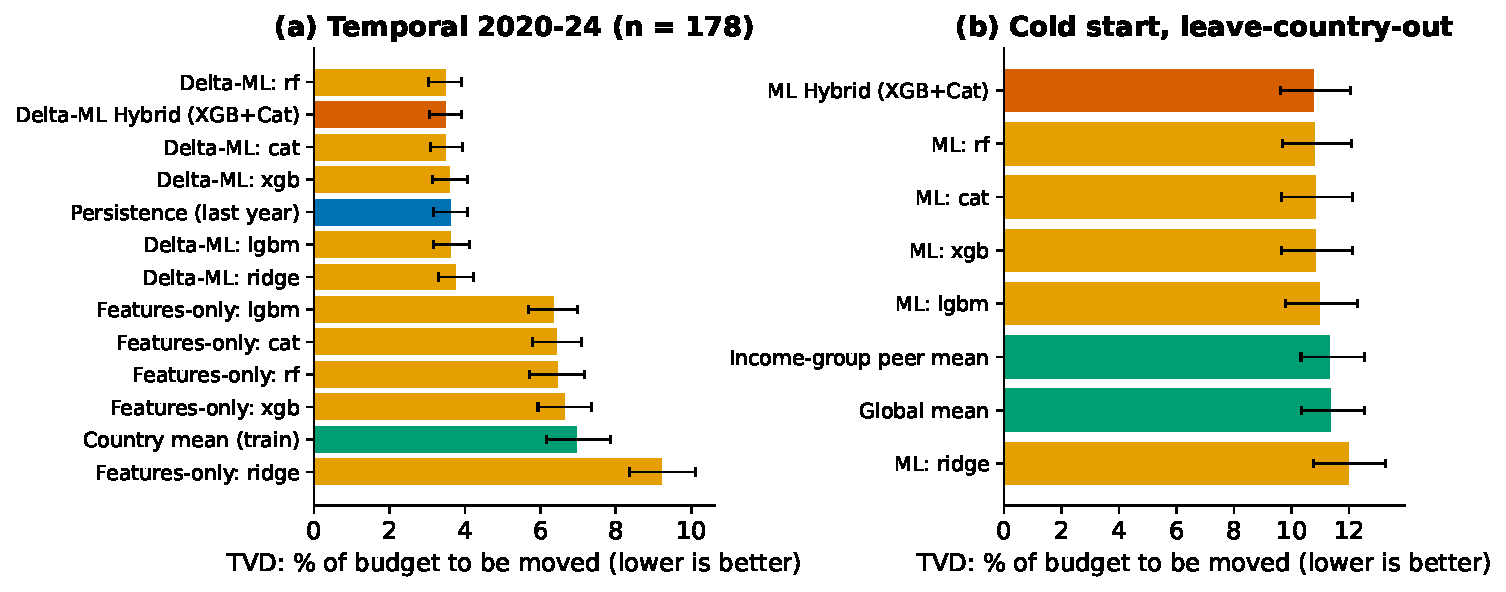
\includegraphics[width=\textwidth]{figures/fig4_main_results.pdf}
\caption{TVD on panel A16 with 95\% cluster-bootstrap CIs: (a) annual update (test 2020--24, $n=178$); (b) cold start (two fold seeds).}\label{fig:main}
\end{figure*}}
\newcommand{\figLime}{\begin{figure*}[!t]
\centering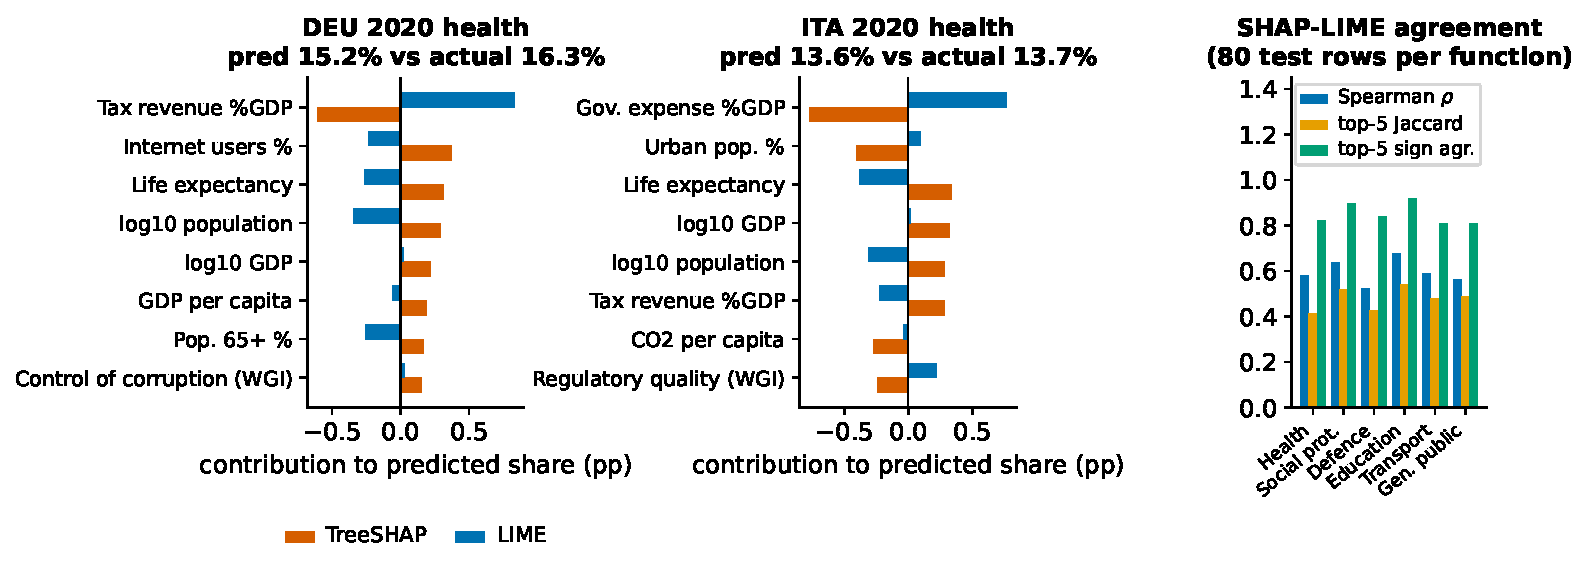
\includegraphics[width=\textwidth]{figures/fig8_shap_vs_lime.pdf}
\caption{SHAP vs.\ LIME: two case studies (signed contributions) and agreement metrics over 80 test rows per function.}\label{fig:lime}
\end{figure*}}


\begin{document}
\title{GovAllocXAI: A Benchmark of Explainable Machine Learning for Predicting Functional Government Expenditure Shares from Official Multi-Country Data}

\author{\IEEEauthorblockN{Aditi H. Joshi\IEEEauthorrefmark{1}, Pranav S. Chaudhari, Gaurav M. Jaypatre, and Digvijay P. Birajdar}
\IEEEauthorblockA{Department of Computer Engineering, Pimpri Chinchwad College of Engineering, Pune, India\\
\{aditi.joshi24, pranav.chaudhari24, gaurav.jaypatre24, digvijay.birajdar24\}@pccoepune.org\\
\IEEEauthorrefmark{1}Corresponding author}}
\maketitle

\begin{abstract}
How much can machine learning add to last year's government budget, and what can peers and explanations tell us when there is no last year? We build a benchmark on official data: \NCofogRows{} COFOG country-years (\NCofogCountries{} economies; Eurostat/OECD; \NTenEcon{} economies with IMF data) and \NWdiRows{} World Bank country-years (\NWdiCountries{} economies). Our earlier semi-synthetic benchmark ($R^2>0.99$) is audited: eleven of its fifteen targets were exact multiples of one series. Last year's allocation is a strong baseline (total-variation distance \ResTVDPersist{} pp); a learned correction using same-year covariates lowers it to \ResTVDHyb{} pp, but the gain averages \AnnSeedMeanGain{} pp over learner seeds and is significant for only \AnnSeedNExcl{} of \AnnSeedN. Without history, a stack and a nearest-economies average beat the income-group mean on the wide panel by about 1.3 pp (Holm $p<0.001$) but not robustly on the 16-function panel, and errors are two to three times larger for lower-income economies. SHAP and LIME agree on direction (sign agreement \AgrSignMean) more than on ranking ($\rho=\AgrRhoMean$).
\end{abstract}
\begin{IEEEkeywords}
government expenditure, COFOG, benchmark, explainable AI, SHAP, LIME, data leakage
\end{IEEEkeywords}

\section{Introduction}
Governments divide limited budgets among health, education, defence and other functions, largely by incremental adjustment. ML can exploit many indicators, but public use demands transparency and human accountability. Prior ML work mostly forecasts aggregate expenditure~\cite{gur2025,dragulin2025}, predicts funding winners~\cite{caravaggio2025,distefano2025}, or relates spending to outcomes~\cite{valle2022,guerrero2022}; functional-spending studies are few and mostly single-country~\cite{santschi2024,radulescu2015,nonato2026,mohith2026}, and SHAP/LIME~\cite{lundberg2017,ribeiro2016} are rarely tested against each other or against known drivers. Our v1 benchmark was semi-synthetic; auditing it showed that its scores were an artefact of the targets. We ask a modest question: how much can ML add to persistence, and what can peers and explanations tell us without history? \textbf{Contributions:} (i) an open, provenance-flagged dataset with official functional targets; (ii) an evaluation protocol with practitioner baselines, cluster-bootstrap intervals and Holm correction~\cite{holm1979}; (iii) a benchmark of learners and negative results, with a stack, a bounded-simplex projection and conformal intervals~\cite{lei2018,angelopoulos2023} as evaluated components; (iv) a quantitative SHAP/LIME evaluation; (v) a leakage audit of the legacy benchmark. We do not claim to be first to predict budgets with ML; to our (non-systematic) search no single prior study covers the conjunction of (i)--(iv) (Table~\ref{tab:gap}).

\section{Related Work}
G\"ur et al.~\cite{gur2025} and Dr\u{a}gulin et al.~\cite{dragulin2025} forecast aggregate expenditure; Santschi et al.~\cite{santschi2024} compare XGBoost/CatBoost with experts on Swiss cantonal accounts; R\u{a}dulescu et al.~\cite{radulescu2015} predict spending by function for five economies; Valle-Cruz et al.~\cite{valle2022} and Guerrero and Casta\~neda~\cite{guerrero2022} link spending to outcomes and SDG gaps. Nonato et al.~\cite{nonato2026} (Brazil, 24 years) model macro outcomes as a function of spending by function and optimise allocations; Mohith et al.~\cite{mohith2026} (India, sectoral allocations; known to us from the abstract only) appears to be the closest allocation-prediction study; Francies et al.~\cite{francies2026} and Kisman et al.~\cite{kisman2026} apply SHAP-type explanations to municipal budgets and defence spending. Explanations are rarely tested against each other or against known drivers, although they can be unstable or manipulable~\cite{alvarezmelis2018,slack2020} and Shapley attributions have conceptual problems~\cite{kumar2020}. Budgeting is classically incremental~\cite{davis1966}, so persistence is the expected benchmark.
\begin{table*}[!t]
\caption{Closest prior work, described by objective attributes. Cells come from the full text where we read it; $^{\dagger}$ = judged from the abstract only. ``Explanations tested'' means that agreement, stability, faithfulness or ground-truth recovery of the attributions was quantified; ``shown'' means attributions were displayed. $^{\ddagger}$ From a secondary summary; the publisher page was not accessible.}\label{tab:gap}
\centering\scriptsize
\renewcommand{\arraystretch}{1.15}
\begin{tabular}{@{}p{2.9cm}p{3.7cm}p{3.1cm}p{2.7cm}p{2.3cm}@{}}
\toprule
\textbf{Study} & \textbf{Setting} & \textbf{Target} & \textbf{Explanation method} & \textbf{Explanations tested}\\
\midrule
G\"ur et al.~\cite{gur2025} & T\"urkiye, monthly 2008--2024 & aggregate expenditure & feature importance (TFT, RF, XGB, MLP) & no\\
Santschi et al.~\cite{santschi2024} & Switzerland, 26 cantons & account groups & none reported & no\\
R\u{a}dulescu et al.~\cite{radulescu2015} & 5 CEE countries & spending by function & none reported & no\\
Valle-Cruz et al.~\cite{valle2022} & 217 countries & spending vs outcomes & none reported & no\\
Guerrero \& Casta\~neda~\cite{guerrero2022} & 140 countries & spending vs SDG gaps & causal framework & n/a\\
Yao \& Zhu~\cite{yao2025} & patient-level insurance cost data & cost of care & SHAP & shown\\
Nonato et al.~\cite{nonato2026}$^{\dagger}$ & Brazil federal, 24 years (+ synthetic) & GDP growth, inflation, Gini given spending by function (allocation by optimisation) & none in abstract & no\\
Kisman et al.~\cite{kisman2026}$^{\dagger}$ & cross-country, 2002--2023 & defence spending (share of GDP, share of spending, per capita) & XAI methods & fidelity/faithfulness reported$^{\ddagger}$\\
Mohith et al.~\cite{mohith2026}$^{\dagger}$ & India, 12 sectors, FY2005--2025 & sector allocations & SHAP, LIME, permutation & not stated\\
Francies et al.~\cite{francies2026}$^{\dagger}$ & Chicago and NYC municipal budgets, 2023--2026 & fund allocations & SHAP, causal model, counterfactuals & composite explainability score (fidelity, interpretability, equity)\\
\midrule
\textbf{This work} & \NCofogCountries{} / \NTenEcon{} economies (COFOG), \NWdiCountries{} (WDI), 2000--2024 & COFOG shares (16 / 10 functions), WDI sector series & TreeSHAP, LIME, KernelSHAP & agreement, stability, deletion, synthetic truth\\
\bottomrule
\end{tabular}
\end{table*}


\section{Data}
\textbf{Sources.} WDI~\cite{wdi} and WGI~\cite{kaufmann2011} provide \NFeatNum{} features; Eurostat~\cite{eurostat_cofog}, OECD~\cite{oecd_table11} and IMF~\cite{imf_gfs} provide general-government expenditure by COFOG function~\cite{un2000cofog}; OECD is used only for economies absent from Eurostat, and the sources agree to a median of \NXsrcMedDiff{} pp on \NOverlapRows{} overlapping rows. \textbf{Panels.} Panel A16 has \NCofogRows{} complete country-years (\NCofogCountries{} economies, 2000--2024), targets being shares of total expenditure of 16 functions plus an unallocated residual (a simplex). Panel A10 (with IMF data) has \NTenRows{} country-years, \NTenEcon{} economies and ten divisions. Panel B has \NWdiRows{} country-years (\NWdiCountries{} economies) with four official series (health, education, defence, R\&D). The data are \emph{executed} spending. \textbf{Policy.} Targets are never imputed; features use $\le$3-year interpolation, then peer-group medians, all flagged and applied before cross-validation (so imputation is transductive); \NFeatModel{} features are used. The legacy v1 dataset is preserved verbatim.

\section{Models and Protocol}
\figArch
\textbf{Learners.} One XGBoost, LightGBM, CatBoost or random-forest regressor per component (fixed hyper-parameters), ridge as linear reference, hybrid $=\tfrac12(\text{XGB}+\text{Cat})$. \textbf{Annual update:} $\hat{\mathbf y}_t=\mathbf y_{t-1}+f(\mathbf x_t,\mathbf y_{t-1})$, so persistence is the null model; because $\mathbf x_t$ are same-year covariates this is a \emph{nowcast}, not a forecast. \textbf{Cold start:} $\hat{\mathbf y}_t=f(\mathbf x_t)$ trained on other economies; the benchmark is the four-class income-group mean. \textbf{Stack:} per component, non-negative-least-squares weights (summing to one) over persistence/peer mean, ridge and XGBoost/CatBoost on raw or log-ratio~\cite{aitchison1986,egozcue2003} targets, fitted on a 2017--19 validation window (annual) or by nested grouped cross-validation (cold start). \textbf{Nearest economies:} inverse-distance-weighted mean composition of the $k=8$ most similar training economies in standardised feature space. \textbf{Conformal:} split-conformal absolute-residual quantiles from out-of-fold training residuals. \textbf{Projection:} $\mathbf a^\star=\arg\min\tfrac12\|\mathbf a-\hat{\mathbf y}\|^2$ s.t.\ $\mathbf 1^{\!\top}\mathbf a=100$, $\boldsymbol\ell\le\mathbf a\le\mathbf u$, solved by bisection and checked against SLSQP. \textbf{XAI:} TreeSHAP~\cite{lundberg2020} and reference LIME~\cite{ribeiro2016}; we measure agreement (Spearman $\rho$, top-5 Jaccard, sign agreement), LIME stability and fidelity, a deletion test (top-3 SHAP vs.\ random features) and a synthetic ground-truth test. \textbf{Evaluation.} TVD $=\tfrac12\sum_k|\hat y_k-y_k|$ in pp (share of budget to be moved; MAE is a constant multiple and is omitted); temporal (train $\le$2019, test 2020--24, a single origin), leave-country-out (6 folds, 2 fold seeds; 5 for robustness) and leave-region-out splits; cluster-bootstrap 95\% CIs over economies~\cite{cameron2008}; Holm correction~\cite{holm1979} over eight cold-start comparisons; stacking follows~\cite{wolpert1992}.

\section{Results}
\textbf{Legacy audit (Fig.~\ref{fig:audit}).} Eleven of fifteen v1 sectors are exact fixed multiples of one series (e.g.\ infrastructure $=2.0\times$ agriculture), so among them all 775 rows share one mix; $k\times$GDP scores $R^2=\LegFormulaRConst$ on them vs.\ \LegXGBRConst{} for XGBoost, and the health column equals an input feature. The $R^2>0.99$ reflects GDP scale, not allocation.
\figAudit

\textbf{Annual update (Table~\ref{tab:A1}, Fig.~\ref{fig:main}a).} Persistence moves \ResTVDPersist{} pp (CI \ResTVDPersistLo--\ResTVDPersistHi); the $\Delta$-hybrid \ResTVDHyb{} pp. For learner seed 42 the paired gain is \ResPairedGain{} pp (CI \ResPairedLo--\ResPairedHi); over five learner seeds it averages \AnnSeedMeanGain{} pp (range \AnnSeedMinGain--\AnnSeedMaxGain) and its CI excludes zero for only \AnnSeedNExcl{} of \AnnSeedN{} seeds. The gain is small and not robust. History-free models are far worse (6.3--9.2 pp). Year-on-year changes in 2020 are only weakly anticipated (health $r\approx\CovTwentyHealth$).
\begin{table}
\caption{Temporal test 2020--24 ($n=178$), one-step-ahead, TVD in percentage points.}\label{tab:A1}
\centering\footnotesize\setlength{\tabcolsep}{3pt}
\renewcommand{\arraystretch}{1.1}

\begin{tabular}{lcc}
\toprule
Method & TVD (pp) & 95\% CI \\
\midrule
Persistence & 3.62 & [3.17, 4.08] \\
Country mean & 6.96 & [6.16, 7.85] \\
Features-only: XGBoost & 6.64 & [5.94, 7.35] \\
Delta-learner: XGBoost & 3.59 & [3.15, 4.06] \\
Delta-learner: CatBoost & 3.50 & [3.08, 3.92] \\
Delta-learner hybrid & 3.48 & [3.06, 3.91] \\
\bottomrule
\end{tabular}
\end{table}

\figMain

\textbf{Cold start (Table~\ref{tab:A2}).} On A16 the hybrid reaches \ResColdHyb{} pp against \ResColdPeer{} pp for the income-group mean (two-seed means); the fold-seed-0 paired gain (\ResColdGain{} pp, CI \ResColdGainLo\ to \ResColdGainHi) is not significant. On the global WDI panel (Table~\ref{tab:B}) leave-country-out $R^2$ is 0.63 for health and 0.60 for R\&D (peer mean 0.31, 0.25; ridge 0.50, 0.53), 0.30 for education and 0.12 for defence; leave-region-out is harder.
\begin{table}
\caption{Cold start: leave-country-out (6 folds $\times$ 2 seeds, mean over seeds), TVD in percentage points.}\label{tab:A2}
\centering\footnotesize\setlength{\tabcolsep}{3pt}
\renewcommand{\arraystretch}{1.1}

\begin{tabular}{lcc}
\toprule
Method & TVD (pp) & 95\% CI \\
\midrule
Hybrid (XGBoost+CatBoost) & 10.77 & [9.60, 12.05] \\
XGBoost & 10.83 & [9.67, 12.12] \\
Income-group peer mean & 11.34 & [10.33, 12.53] \\
Global mean & 11.35 & [10.35, 12.53] \\
ridge regression & 11.98 & [10.75, 13.26] \\
\bottomrule
\end{tabular}
\end{table}


\textbf{Wider coverage and stacking.} On A10 (five fold seeds, Holm-corrected), the stack beats the peer mean by \FSStackTenGain{} pp (CI \FSStackTenLo--\FSStackTenHi, $p=$ \FSStackTenHolm) and the 8-nearest-economies average by \FSKnnTenGain{} pp ($p=$ \FSKnnTenHolm); on A16 the stack's \FSStackSixteenGain{} pp does not survive correction ($p=$ \FSStackSixteenHolm) while the nearest-economies average's \FSKnnSixteenGain{} pp does ($p=$ \FSKnnSixteenHolm). A Dirichlet regression~\cite{ferrari2004} ties the stack on A10 (13.69 vs.\ 13.77 pp). In annual mode the stack is significantly worse than persistence on A10 ($-0.20$ pp, CI $-0.35$ to $-0.03$) and no model beats persistence by a relevant margin. Cold-start error rises with income level (Table~\ref{tab:income}: \ErrHigh{} pp high-income vs.\ \ErrLow{} pp low-income, three economies), an applicability score correlates with it ($\rho=\NovRho$, confounded by income group), and 80\% conformal intervals cover 80.1\% overall but only 47\% (low-income) and 61\% (lower-middle). The error disparity is an equity concern~\cite{mehrabi2021,obermeyer2019}, not a formal fairness test.
\begin{table}
\caption{Cold-start TVD (pp) by income group on the wide panel A10 (50/23/9/3 economies) with the mean applicability (novelty) score. The low-income group has only three economies.}\label{tab:income}
\centering\footnotesize\setlength{\tabcolsep}{3pt}
\renewcommand{\arraystretch}{1.1}

\begin{tabular}{lcccc}
\toprule
Income group & Econ. & Novelty & Peer mean & XGBoost \\
\midrule
High & 50 & 3.38 & 12.5 & 11.4 \\
Upper middle & 23 & 4.05 & 18.3 & 18.5 \\
Lower middle & 9 & 5.65 & 28.1 & 22.0 \\
Low & 3 & 7.67 & 32.1 & 33.4 \\
\bottomrule
\end{tabular}
\end{table}


\textbf{Negative results.} Shock-aware features did not help (2020--21 TVD 4.16 vs.\ 3.89 pp for the baseline; persistence 4.07), persistence was the best deployable method at every horizon of 1--5 years, institutional variables (fiscal rules, elections, IMF programmes) added nothing, econometric panel baselines were significantly worse than persistence, and the IMF source has no COFOG data for 22 of 25 low-income economies. The projection sums to 100\% within $3\times10^{-14}$; tight 1st--99th-percentile bounds clip 37\% of predictions and raise TVD to 3.65 pp, whereas $0.5\times$min to $1.5\times$max clip under 2\% without loss.
\begin{table*}
\caption{WDI global panel, $R^2$. LCO = leave-country-out, LRO = leave-region-out: income-group peer mean vs.\ XGBoost+CatBoost hybrid. \emph{Temporal}: train $\le$2018, test 2019--2024, persistence vs.\ $\Delta$-hybrid with last-year value.}\label{tab:B}
\centering\small
\renewcommand{\arraystretch}{1.1}
\begin{adjustbox}{max width=\linewidth}
\begin{tabular}{lrcccccc}
\toprule
Official series & $n$ & LCO peer & LCO hybrid & LRO peer & LRO hybrid & Persist. & $\Delta$-hybrid \\
\midrule
Health (\%GDP) & 4547 & 0.31 & 0.63 & 0.24 & 0.49 & 0.93 & 0.94 \\
R\&D (\%GDP) & 2212 & 0.25 & 0.60 & 0.23 & 0.48 & 0.99 & 0.99 \\
Education (\%GDP) & 3365 & 0.02 & 0.30 & $-$0.10 & 0.16 & 0.86 & 0.87 \\
Defence (\%GDP) & 3814 & $-$0.02 & 0.12 & $-$0.25 & $-$0.09 & 0.82 & 0.82 \\
Health (\%gov. exp.) & 4547 & 0.28 & 0.43 & 0.25 & 0.14 & 0.89 & 0.90 \\
Education (\%gov. exp.) & 3304 & 0.06 & 0.13 & 0.02 & $-$0.13 & 0.78 & 0.78 \\
Defence (\%gov. exp.) & 3755 & 0.02 & 0.11 & $-$0.24 & $-$0.16 & 0.86 & 0.86 \\
\bottomrule
\end{tabular}\end{adjustbox}
\end{table*}


\textbf{Explainability (Table~\ref{tab:xai}, Fig.~\ref{fig:lime}).} Mean SHAP--LIME Spearman $\rho=\AgrRhoMean$, top-5 Jaccard \AgrJacMean, sign agreement \AgrSignMean; LIME local $R^2=\AgrLimeFit$, re-run stability $\AgrStabMean$. Resetting the top-3 SHAP features moves predictions \AgrFaithMean$\times$ more than random features (range \AgrFaithMin--\AgrFaithMax), which shows that SHAP selects features that matter to the model but is weak evidence (mean replacement; no permutation-importance comparison). In a synthetic test with known drivers both methods recover two of three, and fewer when a correlated copy is added (0.52 TreeSHAP, 0.43 LIME).
\begin{table*}
\caption{Quantitative evaluation of SHAP and LIME (80 random test rows per function). Faithfulness ratio = mean |prediction change| when the three most important SHAP features are reset to the training mean, divided by the same for three random features.}\label{tab:xai}
\centering\small
\renewcommand{\arraystretch}{1.1}
\begin{adjustbox}{max width=\linewidth}
\begin{tabular}{lcccccc}
\toprule
Function & Spearman $\rho$ & Top-5 Jaccard & Top-5 sign agr. & LIME local $R^2$ & LIME re-run $\rho$ & Faithfulness ratio \\
\midrule
Health & 0.58 & 0.41 & 0.82 & 0.47 & 0.92 & 3.1 \\
Social Protection & 0.64 & 0.52 & 0.90 & 0.59 & 0.92 & 3.4 \\
Defence & 0.52 & 0.43 & 0.84 & 0.56 & 0.75 & 3.4 \\
Education & 0.67 & 0.54 & 0.92 & 0.66 & 0.92 & 3.8 \\
Transport & 0.59 & 0.48 & 0.81 & 0.46 & 0.88 & 3.0 \\
General Public Services & 0.56 & 0.49 & 0.81 & 0.36 & 0.75 & 2.0 \\
\midrule
Mean & 0.59 & 0.48 & 0.85 & 0.52 & 0.86 & 3.1 \\
\bottomrule
\end{tabular}\end{adjustbox}
\end{table*}

\figLime

\section{Discussion and Limitations}
The model is a \emph{reference point}, not a recommendation: persistence is hard to beat, and peers help mainly when there is no history. Limits: the annual setting is a nowcast with realised same-year covariates; a single COVID-dominated test window; imputation is transductive; Panel B features include fiscal-envelope variables; current income classification is used for all years; only three low-income economies, so low-income findings are exploratory; the peer baseline has four classes; explanations are associational and refer to the XGBoost member; and no human-subject study has been run. Recommendations inherit historical biases and must never be applied automatically. A declaration of generative-AI use is included in the journal version.

\section{Conclusion}
On official data, last year's allocation is hard to beat (learned gain \ResPairedGain{} pp for one seed, \AnnSeedMeanGain{} on average), peers help without history on a wide panel but not robustly on a narrow one, explanations agree mainly in direction, and shocks need human judgment. We release data, code and the audit, and plan strict forecasting, non-OECD coverage and a human-subject study.

\bibliographystyle{IEEEtran}
\bibliography{references}
\end{document}
